\documentclass[10pt,twocolumn,letterpaper]{article}

\usepackage{cvpr}
\usepackage{times}
\usepackage{epsfig}
\usepackage{graphicx}
\usepackage{amsmath}
\usepackage{amssymb}

\usepackage[breaklinks=true,bookmarks=false]{hyperref}

\cvprfinalcopy % *** Uncomment this line for the final submission

\def\cvprPaperID{****} % *** Enter the CVPR Paper ID here
\def\httilde{\mbox{\tt\raisebox{-.5ex}{\symbol{126}}}}

% Pages are numbered in submission mode, and unnumbered in camera-ready
%\ifcvprfinal\pagestyle{empty}\fi
\setcounter{page}{1}
\begin{document}


%%%%%%%%% TITLE
\title{Helping the Color Blind See Color}

\author{Carolyn Chen\\
Princeton University\\
Princeton, NJ\\
{\tt\small clc4@princeton.edu}
\and
Dorothy Chen\\
Princeton University\\
Princeton, NJ\\
{\tt\small dschen@princeton.edu}
}

\maketitle
%\thispagestyle{empty}

%%%%%%%%% ABSTRACT
\begin{abstract}
   In this paper, we discuss a novel way to combine existing research in computer-assisted vision specific to colorblindness in order to generate re-colorized images, enhancing accessibility specific to the user. We begin be calibrating the user to detect his or her color vision deficiency (CVD). Following this, we re-color the image based on the user’s specific CVD condition. Finally, we assess our results by comparing CVD simulations of the original image and the corrected image. 
\end{abstract}

%%%%%%%%% BODY TEXT
\section{Introduction}

	Genetic photoreceptor disorders are the most common cause of CVD, manifesting in 8\% of Caucasian males, 5\% of Asiatic males, and 3\% of African-American and Native-American males [3]. With this and the female subset being a substantial portion of the population, it is necessary, in our rapidly growing image-based society, to provide an algorithm that can re-color images to make them more accessible to people with CVD. Without such assistive technology, details that are easily seen by people with normal color vision may be completely overlooked by people with CVD due to differences in color perception (see figure \ref{fig:grapes}). Fortunately, there has been some extensive research on color blindness and re-colorization that work towards reducing such differences in perception. While there is clearly no way to eliminate all differences in perception, these methods have been successful in preserving the semantic information of images between people of different color acuity. We therefore aggregate a few existing techniques in our implementation to serve as a proof of concept as well as a new user-specific system by which images are re-colored.

\begin{figure}[h]
  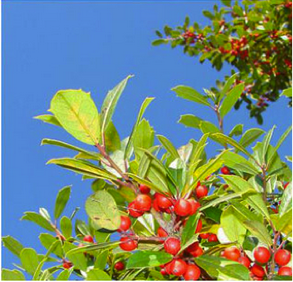
\includegraphics[width=0.22\textwidth]{grapes1.png}
  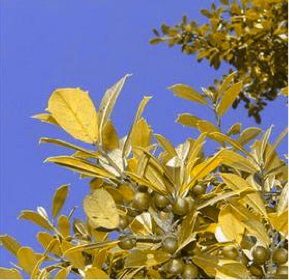
\includegraphics[width=0.22\textwidth]{grapes2.png}
  \caption{(a) is with regular vision; (b) is a simulation of a person with CVD's view}
  \label{fig:grapes}
\end{figure}

Normal color vision eyes contain three fundamental photoreceptor cells. These cells, also known as cone cells, are concentrated in the retina near the blind spot, where they are able to absorb the most light. Each type of cone cell has a different spectral response, where the peak sensitivity regions lie in the long (L), middle (M), and short (S) wavelengths [1]. A genetic CVD will cause either a defect or an absence in these cells. Dichromatic colorblindness, which we focus our work on, occurs when one of these cells is absent [2]. The different types of dichromats are protanopes, deuteranopes, and tritanopes, where the L, M, and S cones are missing (respectively). This essentially reduces the color gamut of the dichromate into two-dimensions, as shown in figure \ref{fig:gamut}.  

\begin{figure}[h]
  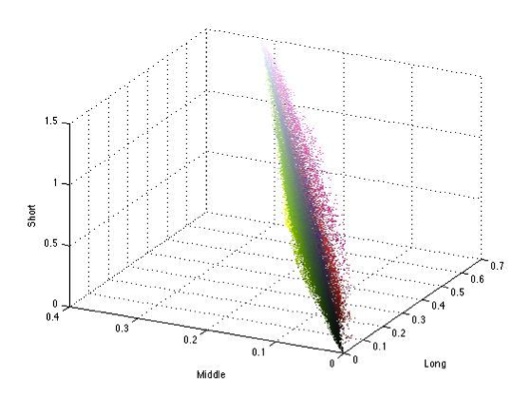
\includegraphics[width=0.22\textwidth]{gamut1.png}
  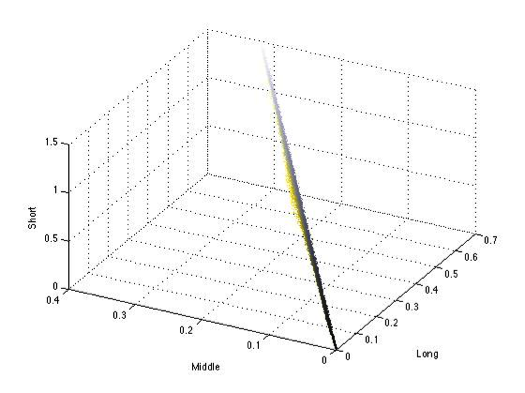
\includegraphics[width=0.22\textwidth]{gamut2.png}
  \caption{(a) LMS representation with regular vision; (b) LMS under simulation of a deuteranope; Source: use getLMSVisualization.m to visualize an image in LMS space. Note the reduction in space}
  \label{fig:gamut}
\end{figure}

	Because there are three different types of dichromatic conditions, we calibrate the user in the beginning of our color-correction tool through an implementation of a technique described in [5]. There are several different ways to determine color-blindness, including the widely used Isihara plates (figure \ref{fig:plate}). However, a more useful diagnostic test, which is used in [5], is the Fansworth Dichotomous test, or the D-15 panel test. The D-15 consists of 15 panels of different colors, all chosen to have the same lightness value, that need to be arranged in order in relation to one static panel. This method has proved to be more effective for scientific research because its results can be quantitatively scored, whereas the Isihara test is simply diagnostic [5]. Because [5] was cited by several papers, we decided to use their method to calibrate our users. Furthermore, not only does it diagnose, but it also provides a way to quantify useful parameters such as the Confusion index, which reveals the severity of colorblindness, and the Selectivity index, which indicates the degree of randomness in the user’s arrangement. These parameters could potentially be used to make our algorithm even more person-specific. 

\begin{figure}[h]
  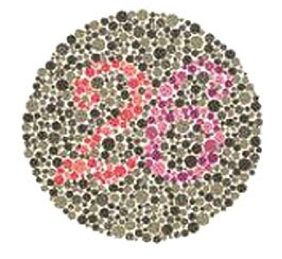
\includegraphics[width=0.4\textwidth]{plate.png}
  \caption{An Isihara plate, used to diagnose different conditions of CVD}
  \label{fig:plate}
\end{figure}

	Following this calibration step is the re-colorization algorithm. The goal of this step is to re-color the image based on the user’s type of CVD so that the user can discern details in the new image that he or she could not do without the enhancement. Authors of [2] propose a re-coloring algorithm that is completely automatic, using a standard four step procedure that involves: 1) finding the key colors of the original image, 2) defining the target distance in the color space to achieve between key colors, 3) an optimization of the mapping of these key colors by minimizing the difference in key color distance between the original and the perceived, and finally 4) re-coloring the image based on the optimization results. The paper claims to exceed previous approaches in both efficiency and effectiveness [2]. It also seemed to have an interesting optimization application, whereas other methods may naively perform a simple stretch of contrast between the colors of an image, which might consequently create great unnaturalness [4]. Because of these reasons and for the purpose of it being a good learning exercise, we chose to attempt to recreate this algorithm for the project. 

	We finish our implementation with an algorithm to simulate color-blindness by following the method described in [1], a paper that is widely cited by works related to this topic. This method makes use of the LMS color space to perform the mapping of colors from the original image to the perceived image. Thus, the algorithm consists of mapping the image to LMS space, mapping the “physiologically undetermined components,” referring to the information marked by the missing cone, to the reduced stimuli surface, and mapping this reduction back to the RGB space. It has been proven to be rather effective in simulating CVD, since people with colorblindness cannot distinguish between the original image and the simulation. We use this algorithm for two purposes: 1) a step in the optimization of the algorithm described in [2] relies on a comparison between a simulation of CVD and the original image, and 2) to serve as a tool for evaluation of this project. 




%------------------------------------------------------------------------
\section{Implementation}

Here, we discuss in more depth the algorithms that we implemented.

%-------------------------------------------------------------------------
\subsection{Calibration}

As discussed in Section 1, we used the algorithm described in [5] to quantify the results of the Farnsworth D-15 panel test for colorblindness. Here, we relay a brief description of our user interface, followed by a summary of the algorithm.

The calibration step involves a simple user interface, where the algorithm randomly scatters the different 15 panels at the beginning, thus forcing the user to order the panels relative to the static blue panel on the left (please refer to the readMe file for instructions to execute quickly without this input step). To submit the response, exit out of the window.

\begin{figure}[h]
  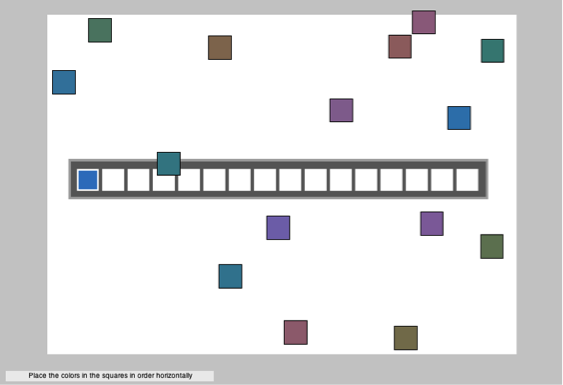
\includegraphics[width=0.5\textwidth]{panel.png}
  \caption{The user interface for calibration}
  \label{fig:panel}
\end{figure}

\begin{figure}[h]
  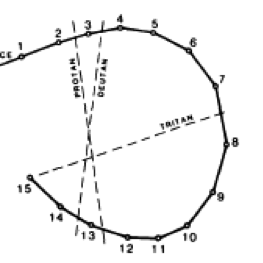
\includegraphics[width=0.22\textwidth]{luv1.png}
  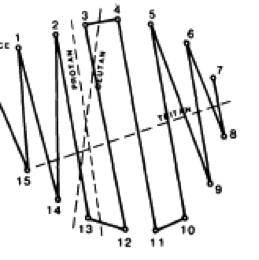
\includegraphics[width=0.22\textwidth]{luv2.png}
  \caption{(a) D-15 ordering of panels for normal vision; (b) ordering for a protanope; Source: [5]. the cross-over in the protanope's ordering}
  \label{fig:luv}
\end{figure}

The different panels, show in figure \ref{fig:panel}, can be mapped to a two-dimensional U*V* plane of the 1976 CIELUV color space, since lightness is held constant among them. This makes for a nice and flat mapping of the ordering of the panels (figure \ref{fig:luv}), where CVDs can be distinguished when orderings cross certain boundaries that distinguish that respective CVD’s confusion locus. What the authors of [5] propose is a way to quantify this ordering by using the color difference vectors between the 15 (or 16 including the starting point) caps.  They then take these vectors to create relative color difference vectors, as shown in figure \ref{fig:compass}, where the length of each vector represents the difference in chroma and the angle represents the difference in hue angle (subsequent of the mapping between U*V*L and LCHuv space) of adjacently placed panels.  

\begin{figure}[h]
  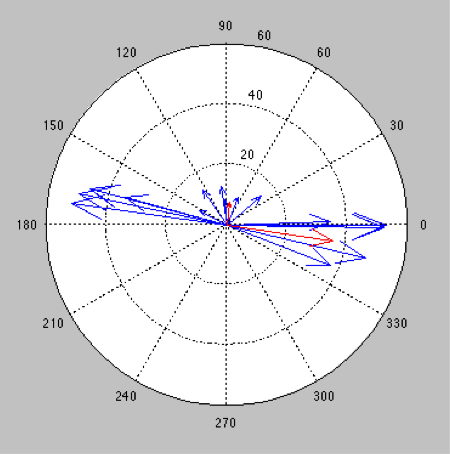
\includegraphics[width=0.5\textwidth]{compass.png}
  \caption{Relative color difference vectors to compute the moment of inertia}
  \label{fig:compass}
\end{figure}

To analyze this data quantifiably, the authors term their approach the Moment of Inertia Method, where each head of the vector has unit mass and the stem is weightless. The method calls to solve for the principal axes of the system that result in the maximum and minimum moments of inertia of the relative difference vectors. This is done by setting the derivative of the inertia with respect to the axis angle to 0, yielding the equation: 

\begin{equation}\label{inertia1}
\tan(2A) = \sum 2U_nV_n / \sum (U_n^{2} - V_n^{2})
\end{equation}

Then, to find the angle of the other axes, it is simply a matter of finding the right angle to A. 
Finally, to find the corresponding moments of inertia, we plug the angles in the following equation:

\begin{equation}\label{inertia2}
I = \sum (V_n\cos(A) - U_n\sin(A))^{2}
\end{equation}

The confusion angle, which allows for a quantitative mapping to the type of CVD, corresponds to the angle that yields the minimum moment of inertia. We used comparison statements based off of Table 1 in the paper, which contained relevant recommended values for each case of dichromacy, to serve as our “diagnosis” for the type of CVD. Furthermore, our code calibrate.m returns other useful parameters such as the Confusion index, calculated by dividing the radius of the major axis by the radius of the smaller axis. This indicates the severity of the colorblindness condition, since theoretically a CVD panel arrangement would consist of several crossings, resulting in large vector lengths in very narrow angle ranges. We further calculate the Selectivity index by dividing the major radius by the major radius of a perfect arrangement, which reveals information about the randomness of the arrangement. These extra parameters may serve to be useful to further customize the user’s experience towards their own unique level of CVD, as we will discuss in section 2.2.d: Gaussian Mapping for Interpolation. 


%-------------------------------------------------------------------------
\subsection{Re-Colorization}

As mentioned in Section 1, we implement the algorithm described in [2]. Here, we summarize the major steps of the algorithm. 

%-------------------------------------------------------------------------
\subsubsection{Image Representation via Gaussian Mixture Modeling}

%-------------------------------------------------------------------------
\subsubsection{Target Distance}

%-------------------------------------------------------------------------
\subsubsection{Solving the Optimization}

%-------------------------------------------------------------------------
\subsubsection{Gaussian Mapping for Interpolation}

The CIELAB space, similar to the CIELUV space, can be mapped to cylindrical coordinates corresponding to lightness, chroma, and hue values (LCH). Because the optimized mapping was simply a rotation in the a*b* plane, as described in the previous steps, the L and C value subsequently remain constant while only the hue angle changes. To calculate the new hue value for each pixel, we first find the difference $M(\mu) -– \mu$ where M is the mapping rotation, meaning we find the hue shift of each Gaussian cluster. Then, depending on the likelihood of a pixel $x_j$ belonging to the ith Gaussian $P(x_j, i)$, we calculate the new hue value, 
$
T(x_j)^{H} = x_j^{H} + \sum\limits_{i=1}^K p(i|x_j, \theta)(M_i(\mu_i)^{H}-(\mu_i)^{H})
$,
which takes into account all the shifts and the posterior probability of the pixel.  Thus, this accounts for a smooth re-coloring, or interpolation, for the adjusted image. 

\begin{figure}[h]
  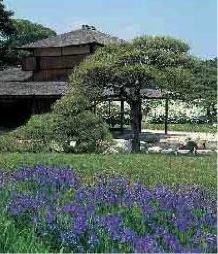
\includegraphics[width=0.22\textwidth]{zen1.png}
  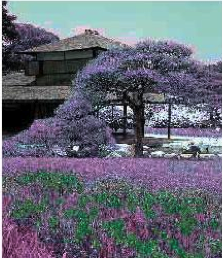
\includegraphics[width=0.22\textwidth]{zen2.png}
  \caption{(a) Original image; (b) Re-colored image for a tritanope}
  \label{fig:zen}
\end{figure}

While the algorithm did not leave room for calibration parameters other than the type of CVD, we hypothesize that there might be a way to incorporate parameters such as severity into the algorithm. For example, for someone who has a deficient amount of L cones as opposed to an absence of all L cones, there will be a response, a reduced response but nevertheless present, of the L cone. Thus, the reduced surface becomes a reduced parallelepiped, and a different mapping can occur. Due to the lack of resources defining this different mapping, we are not able to say with certainty that we have created a re-coloring algorithm that is unique to the user; however, we experimented with a useful parameter returned from calibrate.m, the Confusion Index, which indicates the severity of the CVD. 

Based off of the calibration paper [5], there are approximate values of the C-index that correspond to the different CVD conditions. Thus, in runMe.m, we find the ratio of the retrieved C-index to the known C-index, depending on type. This ratio, upper-capped at one, will determine how we interpolate between the recolored image and the original image: $H(j) = H(j)(1.0-calib.severity) + h_j(calib.severity)$where $H$ is hue and $h_j$ is the recolored hue. *Note, this is not based off of any scientific evidence, as we were unable to access any. The only source that performed an interpolation as well depending on a user parameter was from a Stanford website vischeck that has since closed down. However, we think it is interesting to demonstrate how a user based parameter can affect the outcome, as seen in the following figures. 

\begin{figure}[h]
  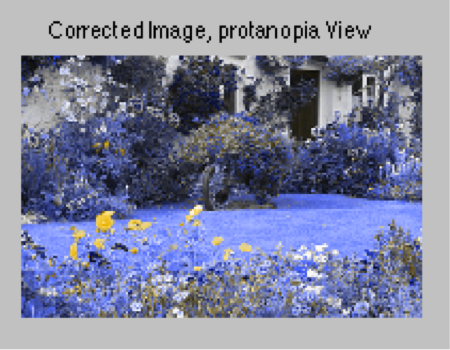
\includegraphics[width=0.22\textwidth]{sev1.png}
  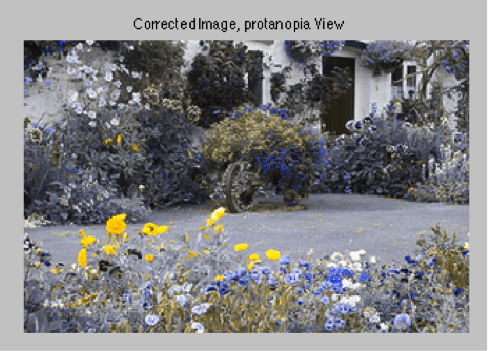
\includegraphics[width=0.24\textwidth]{sev2.png}
  \caption{(a) Corrected image for a protanope of severity 1.0; (b) Corrected image for severity 0.5; Note the difference in the brightness of color, where in (a), the contrast between the grass and the yellow flowers is much more accentuated}
  \label{fig:sev}
\end{figure}

%-------------------------------------------------------------------------
\subsection{Simulation}

We implemented the simulation algorithm described in the prevalently cited paper [1]. This can be broken down into three transformation steps, which are described below.

(1) Translate the pixel value to LMS space. This is relatively straightforward, as it is a simple matrix multiplication: $Q = TV$, where Q is the resultant LMS values corresponding to the current pixel, V is the RGB equivalent, and T is composed of the LMS tristimulus values of the Cathode Ray Tube (CRT) monitor used in the paper. The LMS tristimulus values, or the values of the three primaries at maximum intensity, are dependent on the monitor. However, since we did not have access to a spectroradiometer, we were unable to calculate our own LMS tristimulus values corresponding to our personal computers. Thus, we made the assumption that the difference in values between the example that is given in the paper, the Hitachi Model CM2086A3SG Monitor, and our own is minimal and used those values to compose our T and consequently $T^{-1}$ matrix: 
\[ T = \left| \begin{array}{ccc}
0.1992 & 0.4112 & 0.0742 \\
0.0353 & 0.2226 & 0.0574 \\
0.0185 & 0.1231 & 1.3550 \end{array} \right|.\]

(2) 	Apply the simulation algorithm. Because we are given the maximum limits of the RGB channels in LMS space, we can define a parallelepiped in LMS space that defines all the colors that can be produced by the specific monitor (see figure \ref{fig:para} for a nice illustration).  Within this space, depending on the type of colorblindness, is the parallelogram that defines the reduced stimuli surface, since, as we recall, dichromacy occurs when one of the LMS cones is lacking. To map a normal pixel to a simulated pixel, the algorithm projects that value to its corresponding position on the reduced stimuli surface. 

\begin{figure}[h]
  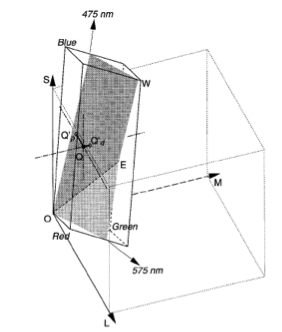
\includegraphics[width=0.5\textwidth]{para.png}
  \caption{Reduced stimuli surface for a protanope; Source: [1]}
  \label{fig:para}
\end{figure}

Depending on the position of the current pixel with respect to the neutral axis OE, as seen in figure \ref{fig:para}, which divides the reduced stimuli surface into two parts, the monochromatic anchor stimulus, in nanometers, is one of two values. In other words, a certain wavelength corresponding to an invariant hue can be assigned as the anchor value for a reduced color, acting as one of two vectors to define the half-plane the pixel is projected down to. The other vector that defines this plane is E, the brightest possible metamer of the equal energy stimulus on the monitor. Here, we assume, due to lack of knowledge of the monitor, that E is represented as [1;1;1] in RGB, or equivalently White, a metamer for white light from the monitor. These two vectors define the plane, and since the cross-product of the two will be orthogonal to the vector defining the new projected pixel, we can solve a series of equations to obtain the mapping of the simulated pixel, taking into account also the loss of information from one of the LMS dimensions. 
(3) 	Re-map back the LMS values to pixel values in RGB space.  This step was simple enough, involving a straightforward transformation using the inverse T matrix. To speed up the simulation algorithm, we factored out a lot of code. This was essential because the optimization portion of the algorithm relied on the simulation as well. 

%------------------------------------------------------------------------
\section{Results and Evaluation}

It was difficult to find a sufficient number of subjects to test our program on to make any significant claims on its success. However, as many of our sources used as well for their evaluation metrics [2-4], we evaluated the “success” of the implementation based on a comparison between the simulated views of the original image and the re-colored image. Through this qualitative sketch, an image would be perceived as a “success” if, between the two simulated images, the re-colored image contained more information regarding color contrast versus the original image. Another possible way to evaluate the results, quantifiably, would be to use the Gaussian Mixture Modeling approach used in the re-colorization step to detect key colors in both the simulation of the original and the simulation of the re-colored. If the ratio between the re-colored and the original is greater than 1, then that means that there was a gain in information.  ADD STUFF HERE IF ACTUALLY DO IT

Below are results that demonstrate the “success” of the algorithm introduced by [2]. Here we can clearly see the improvement in the Isihara plate, where without the color-correction, the number is invisible to the viewer. Testing on natural images, we can see there is an improvement there as well. In the image of the fruit vendor, the simulated original image appears to be selling one long pile of oranges behind the bananas. However, in the re-colored image, the algorithm illuminates the different piles so the viewer can see there are actually three different piles of fruit. 

\begin{figure}[h]
  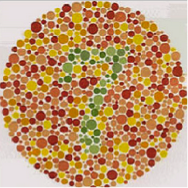
\includegraphics[width=0.23\textwidth]{isihara1.png}
 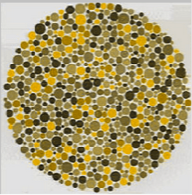
\includegraphics[width=0.23\textwidth]{isihara2.png}
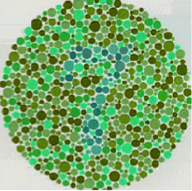
\includegraphics[width=0.23\textwidth]{isihara3.png}
  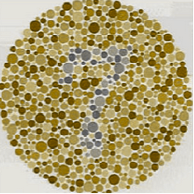
\includegraphics[width=0.23\textwidth]{isihara4.png}
  \caption{(top-left) Original image; (top-right) Original image, protanope view; (bottom-left) Corrected image; (bottom-right) Corrected image, protanope view, 7 now visible}
  \label{fig:isihara}
\end{figure}

\begin{figure}[h]
  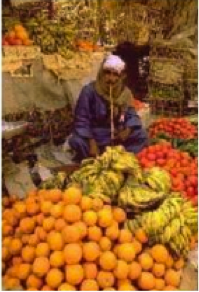
\includegraphics[width=0.23\textwidth]{fruits1.png}
 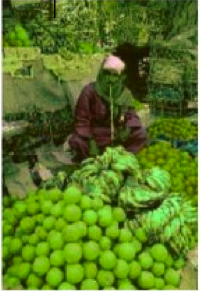
\includegraphics[width=0.23\textwidth]{fruits3.png}
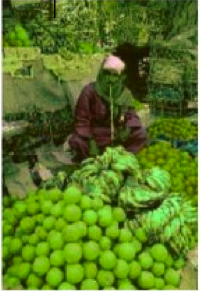
\includegraphics[width=0.23\textwidth]{fruits2.png}
  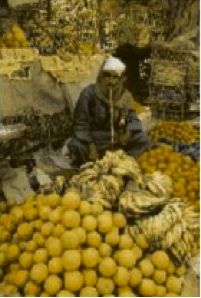
\includegraphics[width=0.23\textwidth]{fruits4.png}
  \caption{(top-left) Original image; (top-right) Original image, deuteranope view; (bottom-left) Corrected image; (bottom-right) Corrected image, protanope view, three piles now visible}
  \label{fig:fruits}
\end{figure}

An interesting result from our implementation was the re-colored version of the red flower. As seen in figure \ref{fig:flower}, re-coloring changed the leaves to blue in simulation. Remarkably, the paper that we followed reported a change in, rather, the flower to blue after the re-colorization. This may be due to the algorithm being stuck in a local minima…? NEED YOUR HELP HERE ☺ 

\begin{figure}[h]
  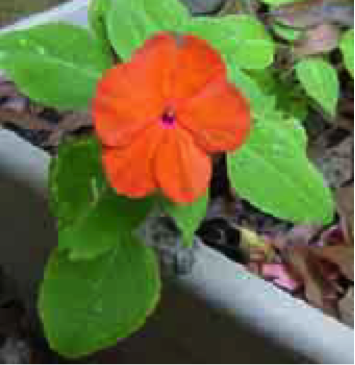
\includegraphics[width=0.23\textwidth]{flower1.png}
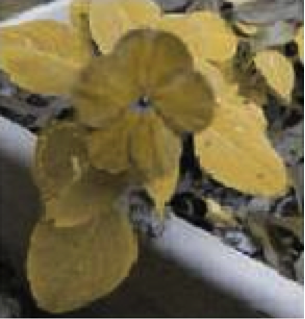
\includegraphics[width=0.23\textwidth]{flower2.png}
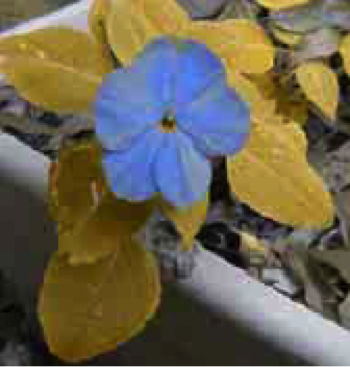
\includegraphics[width=0.23\textwidth]{flower3.png}
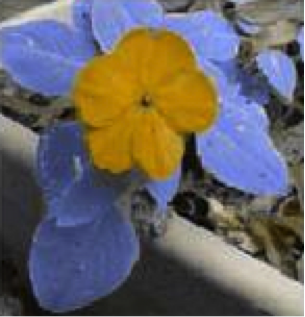
\includegraphics[width=0.23\textwidth]{flower4.png}
 \caption{(top-left) Original image; (top-right) Original image, deuteranope view; (bottom-left) Simulated corrected image ([2]); (bottom-right) SImulated corrected image (ours)}
  \label{fig:flower}
\end{figure}

	After implementing the algorithm, we see obvious practical problems with it. For one, it is non-deterministic, as the paper admits that it needs to be performed several times, taking the solution with the least error, to find the best re-colorization. This problem is due to the optimization getting stuck in local minima. XX MAYBE ADD SOMETHING HERE? Furthermore, if there were more time, it would have been interesting to compare the results of another re-colorization algorithm, such as in (Khun), that claims to preserve the “naturalness” of the image. Here, we see, as in the garden image, that results can sometimes seem very unnatural. 

\begin{figure}[h]
  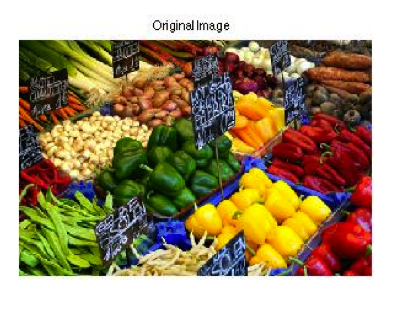
\includegraphics[width=0.23\textwidth]{peppers2.png}
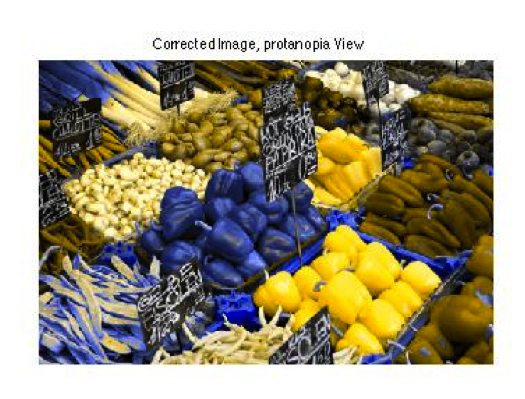
\includegraphics[width=0.23\textwidth]{peppers.png}
 \caption{(a) Original image; (b) Simulation of corrected image, protanopic, note some of the unnaturalness}
  \label{fig:peppers}
\end{figure}

The runtime of the re-colorization step is $O(KN)$ for key color extraction and re-coloring, and $O(K^{2})$ for optimization, where $K$ is the number of clusters and $N$ is the number of pixels. Simulation is $O(N)$. This reflects the notable increase in time when a greater number of clusters is considered. For example, one of the largest images in our bank is 312 by 467 pixels in dimension, a little over the biggest image reported by the paper [2]. Our re-coloring implementation takes 23.097 seconds to run for a Gaussian Mixture Model of size 6. For a size of 12, it runs for 111.496 seconds. This runtime is too slow to do real-time processing, although this application would have been useful for other media such as video. Our runtime is about four times slower than the results reported in [2], the reason being that we run more iterations in our version to accommodate for occasional non-conversion.  We think this is a fair trade-off.  The algorithm described in [4] suggests some meddling with the GPU to make computation more efficient, but we did not have enough time to experiment with that. 

%------------------------------------------------------------------------
\section{Conclusion}

In this paper, we implemented a user-calibrated system to re-color images for people with CVD. We first employed the Farnsworth D-15 panel test to “diagnose” the user, basing this off of the quantifiable method described in [5]. Then, we followed the algorithm described in [2] to perform the re-colorization of the image. Our evaluation of this method showed that, while it does produce noticeable improvement, it sometimes lacks in naturalness and is not efficient enough to apply to real-time processing. In order to simulate the differences between the original and re-colored images as viewed by the person with CVD, we implemented the simulation algorithm suggested by [1]. Future work on this topic should be spent towards creating more “natural” re-colorized images as well as searching for a more efficient way to process the images.

%------------------------------------------------------------------------
\section{Acknowledgements}

We thank Professor Xiao as well as the TAs of COS 429, Pingmei Xu, Brian Matejek, and Shuran Song. This work has been supported by Princeton University’s Department of Computer Science. 


%------------------------------------------------------------------------
\section{References}

{\small
\bibliographystyle{ieee}
\bibliography{egbib}
[1] Brettel, Hans, Françoise Viénot, and John D. Mollon. "Computerized Simulation of Color 
Appearance for Dichromats." Journal of the Optical Society of America A 14.10 (1997): 2647-655. 

[2] Huang, Jia-Bin, Chu-Song Chen, Tzu-Cheng Jen, and Sheng-Jyh Wang. "Image Recolorization for the Colorblind." IEEE (2009): 1161-164. 

[3] Jefferson, Luke, and Richard Harvey. "An Interface to Support Color Blind Computer Users." ACM (2007).

[4] Kuhn, Giovane R., Manuel M. Oliveira, and Leandro A. Fernandes. "An Efficient Naturalness-Preserving Image-Recoloring Method for Dichromats." IEEE (2008).

[5] Vingrys, Algis J., and P.Ewen King-Smith. "A Quantitative Scoring Technique For Panel Tests of Color Vision." Investigative Ophthalmology \& Visual Science 29.1 (1988): 50-63. 

}

\end{document}
